
\documentclass[a4j,10pt]{jsarticle}
\usepackage{layout,url,resume}
\usepackage[dvipdfmx]{graphicx}
\pagestyle{empty}

\begin{document}
%\layout

\title{2016年 秋 村井研 TERM中間\\
SMTP-STS : SMTP Strict Transport Security
\\を用い暗号化された電子メール通信経路の確立とその実装}

% 和文著者名
\author{
    尾崎周也 (shuya) \thanks{慶應義塾大学 総合政策学部}
    \\shuya@sfc.wide.ad.jp
    \and
    親 中島博敬 (nunnun) \thanks{慶應義塾大学 政策・メディア研究科}
    \\nunnun@sfc.wide.ad.jp
}


% 和文概要
\begin{abstract}
\\
本研究はSMTPにおけるクライアント-MTA間の通信において中間者攻撃の脆弱性が存在する問題に着目し,IETF UTA Working Groupで審議中のSMTP STS(SMTP Strict Transport Security)\cite{draft}をJavaScriptにて実装する.実装物と既存実装物の相互運用テストを行うとともに,その有用性と問題点を考察する.
\end{abstract}

\maketitle
\thispagestyle{empty}

\section{背景}

SMTPはWWW以前から使用されているメール配送プロトコルの標準技術だ.SMTPは当初の仕様から今日に至るまで改善が続けられており現在も使用されている.電子メールは配送されるまでに1つまたは複数のMTAを経由して配送されるが,その通信経路は必ずしも暗号化されていない問題がある.[図1]
\begin{figure}[htbp]
 \begin{center}
      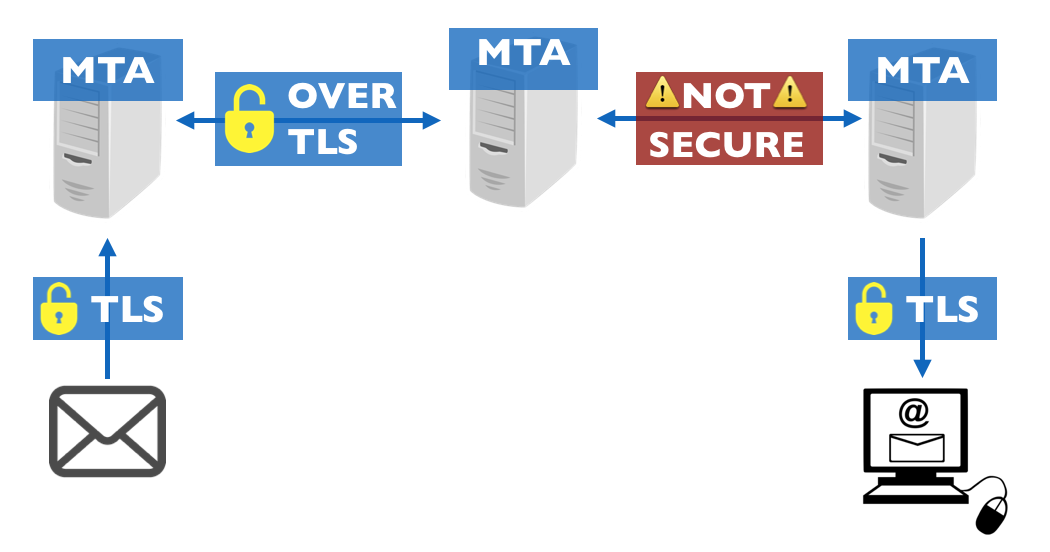
\includegraphics[width=7cm]{figure1.png}
      \caption{電子メールの配送経路}
    \end{center}
\end{figure}

STARTTLS拡張で通信経路の暗号化は行われるが,日和見暗号化であるため能動的な攻撃を防ぐことは難しい.つまり中間者攻撃には脆弱である.ここに2つの攻撃例を示す.

\begin{itemize}
\item POODLE攻撃 
\item DNS Poisoning
\end{itemize}

\subsection{POODLE攻撃}
POODLE攻撃とは暗号化された通信から脆弱性をつき情報を盗み出す攻撃だ.現在はトランスポート層における通信秘匿技術としてTLS1.2の使用が推奨されておりほとんどのサーバやブラウザはTLS1.2に対応している.しかし全てのサーバ,ブラウザが対応しているとは限らない.そのため互換性を確保するために古い暗号方式での通信リクエストを受ける場合がある.その際,SSL3.0のようなセキュリティホールが既知化したプロトルで通信をすることが可能となる.このプロトコルのダウングレードを悪用して中間者攻撃を行うのがPOODLE攻撃である.

\subsection{DNS Poisoning}
DNS Poisoningも考えられる.DNS応答が偽造・改竄されているサーバに接続した場合,ユーザは意図しない接続先に誘導される.DNSSECで正当性が証明されない限りそのサーバが意図したものかユーザは判断することができない.

\section{研究目的}

以上から本研究では中間者攻撃に脆弱であるSMTPの現状を問題とし,SMTP-STSによるセキュアなMTA間通信を実現することを目的にする.


\section{関連技術}

関連技術は2点あげられる.

\subsection{HTTP Strict Transport Security (HSTS)}
HSTSはWebサーバがブラウザに対して現在のアクセス以降はHTTPではなくHTTPSでの接続を強制するセキュリティ機構である.SMTP-STSの考えはこれに基づく.

\subsection{DNS-based Authentication of Named Entities(DANE)}
DANEはドメイン(DNS)とそれに証明書を発行する証明局との紐付けを明確化するセキュリティ機構だ.DANEによってサーバの応答の正当性を担保することができる.

\section{提案手法}

本研究では上記の問題を解決するためにSMTP-STSを実装する.SMTP Strict Transport Security (SMTP-STS)はSMTPの中間者攻撃への脆弱性から検討されている新しいセキュリティ機構であり,IETF UTA Working Groupで審議中だ.\cite{draft}SMTP-STSの技術的特徴は2点に集約される.

\begin{itemize}
\item メールプロバイダが特定の認証(DANE)が有効なTLS接続上でメールの配送ができることを宣言する.
\item 通信経路が暗号化されていなかった場合は報告する,またはメールの受け取りを拒否する.
\end{itemize}

\section{実装}

実装は特定の機能,TLS接続の認証の部分にしぼったMVPを実装する予定だ.また2つの方法を考えている.

\begin{enumerate}
\item Harakaプラグインとして実装する
\item 既存実装をJavaScriptで再実装する
\end{enumerate}

HarakaとはNode.jsで実装されたOSSのSMTPサーバであり,この拡張機能としての実装を目指す.既存実装を再実装するという点では,現在GitHub上にある実装物(go,pythonの2つ)は最新のドラフトを反映していないものだ.本研究ではドラフトを反映させた実装を目指す.

\section{評価}

評価は実装物と既存実装間で疎通がとれるかに設定する.

\section{展望}

先述したように本研究ではMVPのみの実装を行う.MVPのみを実装する理由はSMTP-STSの土台技術であるDNSSECが正常動作しているサーバが現時点ではまだ少ないためだ.\cite{dnssec}本研究のMVPと既存実装との疎通が確認された後,ドラフトに従いSMTP-STSの他の機能の実装を行う予定だ.

\section{スケジュール}

\begin{itemize}
  \item12月中旬まで : ドラフトを踏まえた要件定義を行う
  \item 正月まで : プログラムの設計を行う
  \item 1月下旬まで : TLS接続の認証部部分の実装を行う
  \item 発表まで : 評価・発表準備を行う
\end{itemize}

\begin{thebibliography}{9}
\bibitem{draft}
D. Margolis et al, “SMTP Strict Transport Security”, Internet Draft, March 2016.\\
\url{https://tools.ietf.org/html/draft-margolis-smtp-sts-01}

\bibitem{dnssec}
DNSSEC name and shame!\\
\url{ https://dnssec-name-and-shame.com/}
\end{thebibliography}

\end{document}
% end of file
